\section{Production of resonance with strangeness}

The Quark Model, proposed independently by Murray Gell-Mann and Yuval Ne?eman in 1964 \cite{cite:gellmann}, enables the classification of hadrons in terms of their constituent quarks. In this model, the lighter mesons and baryons are representations of an SU$_{f}$(3) group, whose fundamental representation is the three dimensional vector (u, d, s). These are the three lighter quarks whose characteristics are reported in Table ref{table:quark}. 

\begin{table}[h!]
\centering
\begin{tabular}{lclclc|c|}
\hline
Light flavor &   d  & u  & s \\
\hline \noalign{\smallskip}
Baryon number (B) &  +1/3     & +1/3  &  +1/3\\
Electric charge (Q) &   -1/3     &  +2/3 &   -1/3 \\
Isospin (I)               &   -1/2     &  +1/2 &     0\\
Strangeness (S)     &     0   & 0 & -1\\
mass (\mmass)   &    2.3$_{-0.5}^{+0.7}$    & 4.8$_{-0.3}^{+0.5}$  &  95$\pm$5\\
\hline\noalign{\smallskip}
\noalign{\smallskip}
\end{tabular}
\caption{Quantum numbers and masses associated to the three lighter quarks: u, d and s}\label{table:quark}
\end{table}

The hadronic state are obtained from the decomposition of the following scalar products of the fundamental representations of the group: \\

Meson (q$\bar{q}$) 3 $\bigotimes$ $\bar{3}$ =  1 $\bigoplus$ 8 \\

Baryon (qqq) 3 $\bigotimes$ 3 $\bigotimes$ 3  =  10$_{S}$ $\bigoplus$ 8$_{M}$ $\bigoplus$ 8$_{M}$ $\bigoplus$ 1$_{A}$ \\

For the baryons without $c$ or $b$ qaurk, flavor and spin may be combined in an approximate flavor-spin SU(6), in which the six basic states are d $\uparrow$, d $\downarrow$, $\cdot$ $\cdot$ $\cdot$, s $\downarrow$ ($\uparrow$, $\downarrow$ = spin up, down). Then the baryons belong to the multiplets on the right side of \\

6 $\bigotimes$ 6 $\bigotimes$ 6  =  56$_{S}$ $\bigoplus$ 70$_{M}$ $\bigoplus$ 70$_{M}$ $\bigoplus$ 20$_{A}$ \\

Here, the 56 representation can be decompose in an octet ($J^{P}$ = 1/2$^{+}$) and a decuplet ($J^{P}$ = 3/2$^{+}$), as can be seen in Figure \ref{fig:octet} and Figure \ref{fig:decuplet}.

\begin{figure}[htbp]
\begin{center}
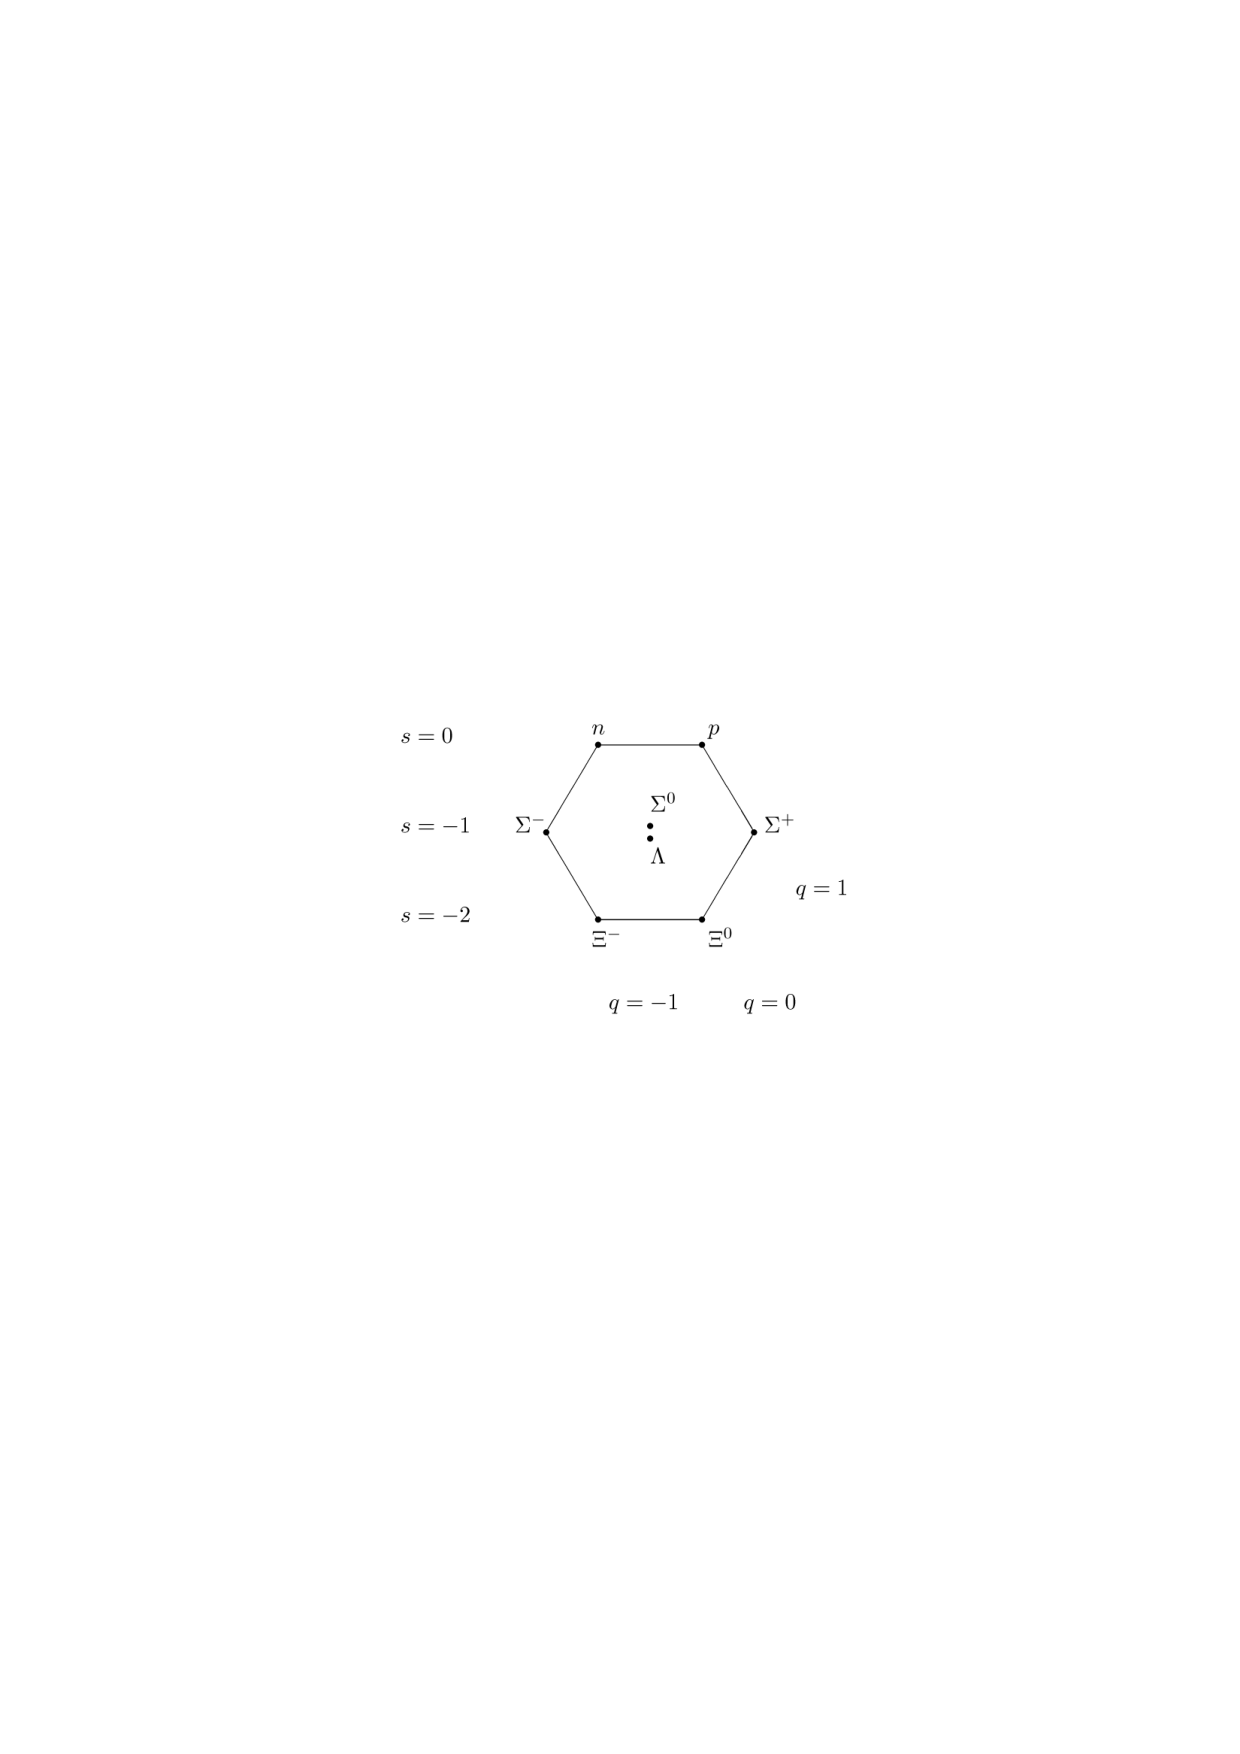
\includegraphics[width=10.cm]{./Version1/FigChapter3/Octet}
\caption{ The $J^{P}$ = 1/2$^{+}$ ground state baryon octet}
\label{fig:octet}
\end{center}
\end{figure}

\begin{figure}[htbp]
\begin{center}
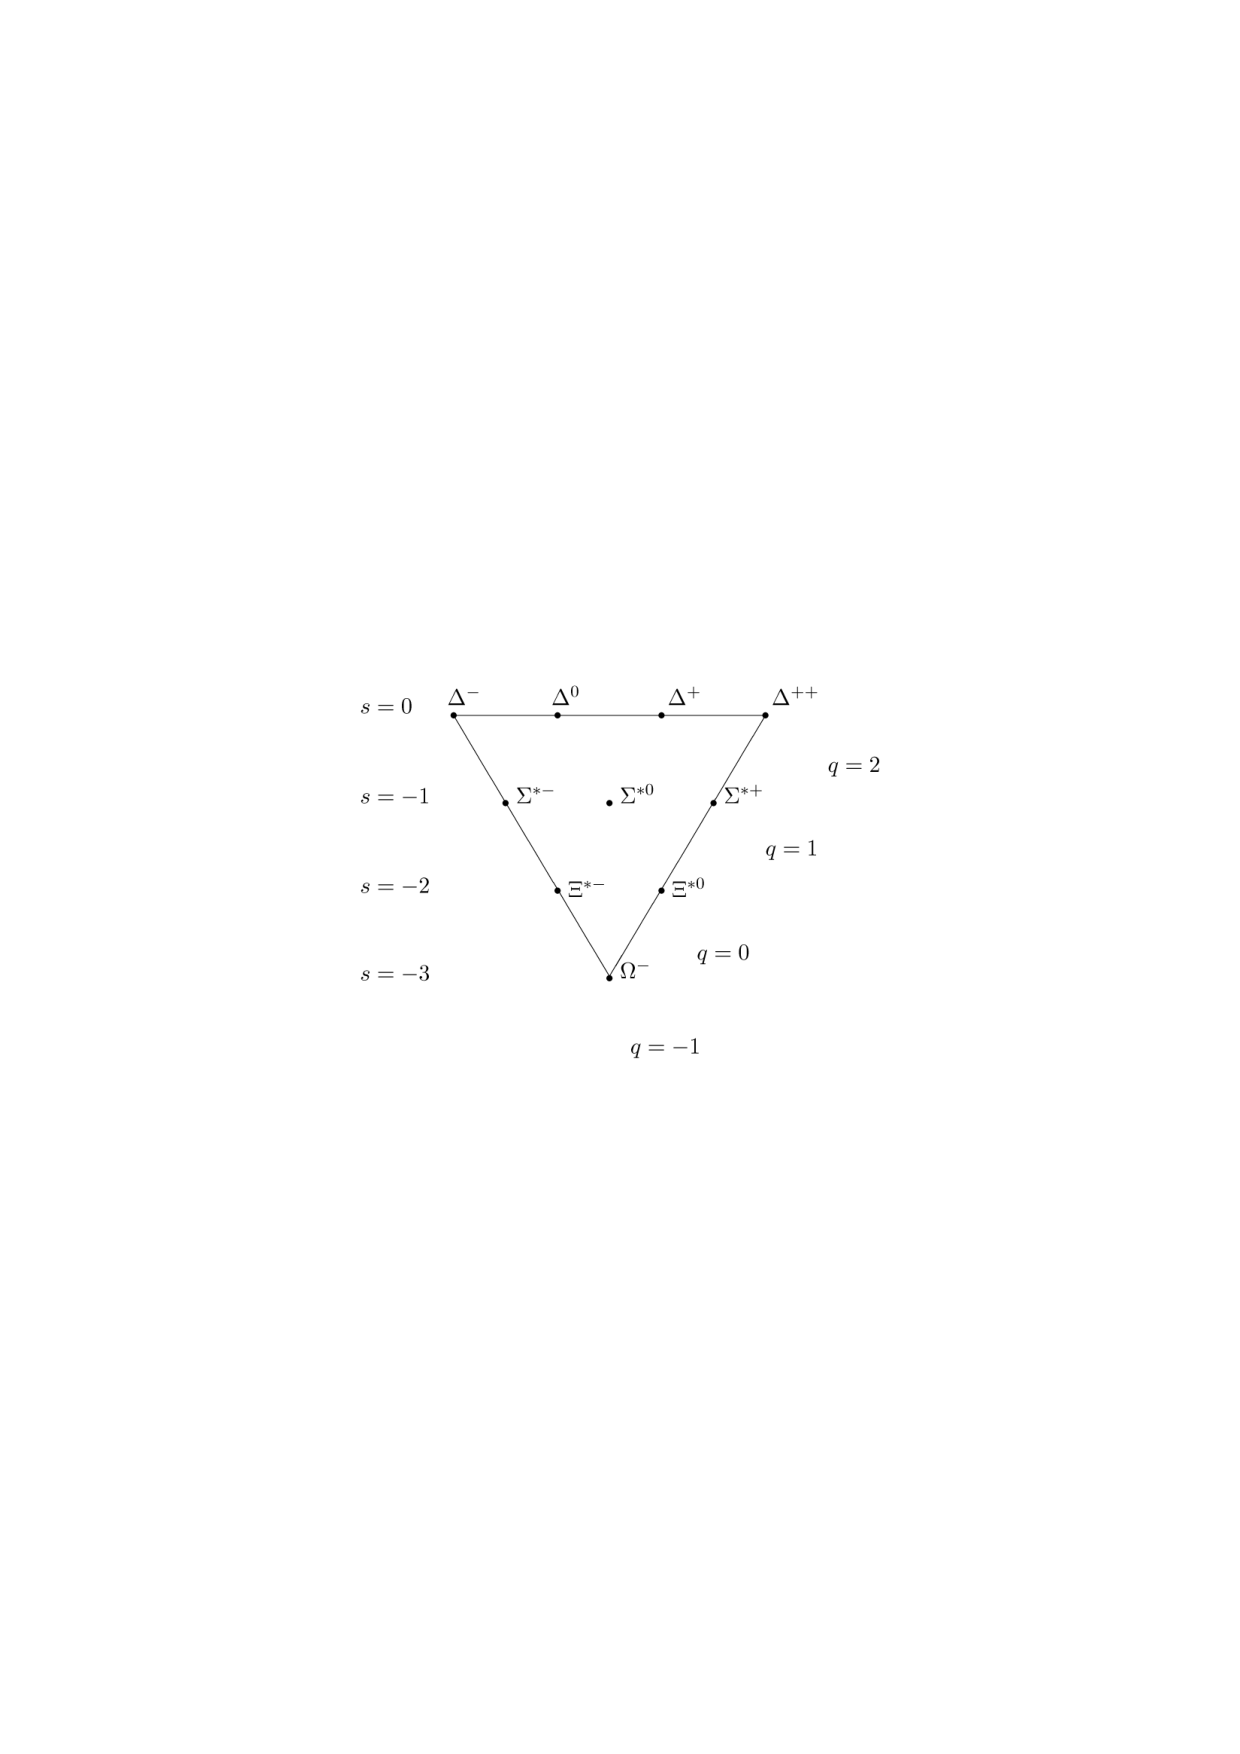
\includegraphics[width=10.cm]{./Version1/FigChapter3/Decuplet}
\caption{ The $J^{P}$ = 3/2$^{+}$ baryon decuplet}
\label{fig:decuplet}
\end{center}
\end{figure}

Among the hadrons, the special family of particles that contain at least one strange quark but not heavier quarks (like charm or bottom), are called hyperons. These are: the $\Lambda$(uds), the triplet $\Sigma^{+}$(uus), $\Sigma^{0}$(uds), $\Sigma^{-}$(dds), the doublet $\Xi^{-}$(dss), $\Xi^{0}$(uss) and the $\Omega$(sss) and the corresponding antiparticles. $\Xi$ and $\Omega$ are the only hyperons containing more than one strange quark, hence they are called multi-strange baryons. 
Resonances shown in Figure ref{fig:decuplet} having * with its name (e.g. X*$^{\pm}$) are particles with higher mass than the corresponding ground state particle with the same quark content. 
Different resonances with different lifetimes can probe different stages of the fireball expansion. The lifetime of some short-lived resonances is reported in Table \ref{table:rsnptl}. The ratios between resonances and stable hadrons can be compared for resonances with different lifetimes and provide insights on the role of the re-scattering effect between the two freeze-out phases.


\begin{table}[h!]
%\centering
\begin{center}

\begin{tabular}{|c|c|c|c|c|c|c|clc|c|c|}
\hline
Particle & $\rho$(770) & $\Delta$(1232) &K*(892) & $\Sigma$(1385) &$\Lambda$(1520) & $\Xi$(1530)& $\Phi$(1020)\\
\hline
Lifetime[c$\tau$] &  1.3 fm &1.7 fm & 4.0 fm& 5.5 fm& 10.3 fm & 22 fm& 46 fm\\
\hline
\end{tabular}
\caption{Lifetime of hadronic resonances}\label{table:rsnptl}
\end{center}
\end{table}



In the following, a general overview of the role of the strange quark within the QGP studies with heavy-ion collisions is given.
%First of all, no net strangeness is present in the colliding objects before collision. Indeed, both the nucleons, proton and neutron, contain only u and d quarks among their valence quarks. All the net strangeness present in the final states (particles) is then created during the collision, and therefore the s quark plays an interesting role in the study of particle production.
And  importance of the measurement of resonance is explained as probe of properties in hadronic phase between the chemical($T_{ch}$) and the kinetic freeze-out($T_{kin}$). 



\subsection{Strange quark and hyperons}
  
The original interest in the strangeness in the context of the QGP comes from an idea by Johann Rafelski and Berndt M$\ddot{u}$ller. In 1982, they suggested a possible signature for the formation of a QGP in a heavy-ion collision \cite{cite:strangeness}. The key argument, at a fixed collision energy, rests on the different production mechanism of the s quark within two different systems:
\begin{description}
\item[1. Hadron Gas (HG)], where the degrees of freedom are the hadronic ones, as quark and gluons are confined
\item[2. QGP], where the degrees of freedom are partonic ones, with quarks and gluons free with respect to each other
\end{description}


The mass of the hadrons is only partly due to the mass of the constituent valence quarks.

 Naively speaking, the quarks ?dress up? due to the strong interaction that keeps them confined. Once they are free, as in a QGP, the quarks recover their bare masses. It was predicted that, if the QGP is formed, an enhancement of the strange quarks should occur, because the production of $s\bar{s}$ pairs becomes easier due to the lower energy needed. When the QGP cools down, these strange quarks eventually recombine into hadrons favoring also an enhancement of the number of strange hadrons. This effect is larger for hadrons with higher strangeness, with the following scaling for the number type: \\

$N_{\Omega} >  N_{\Xi} > N_{\Lambda}$

where $N_{\Omega}$, $N_{\Xi}$, $N_{\Lambda}$ are the number of produced $\Omega$, $\Xi$ and $\Lambda$. A certain enhancement of strange hadrons can occur also in a hadron gas system, but the processes of hadronisation in this case are relatively easy for K and  $\Lambda$. and progressively harder for hadrons with higher strangeness, hence the relation would be: \\

$N_{\Omega} <  N_{\Xi} < N_{\Lambda}$.

The production of multi-strange hadrons with respect to pp - like collisions is considered to be a signature of the formation of the QGP and it was observed at SPS, RHIC and LHC. \cite{cite:strangePbPb}


\begin{figure}[htbp]
\begin{center}
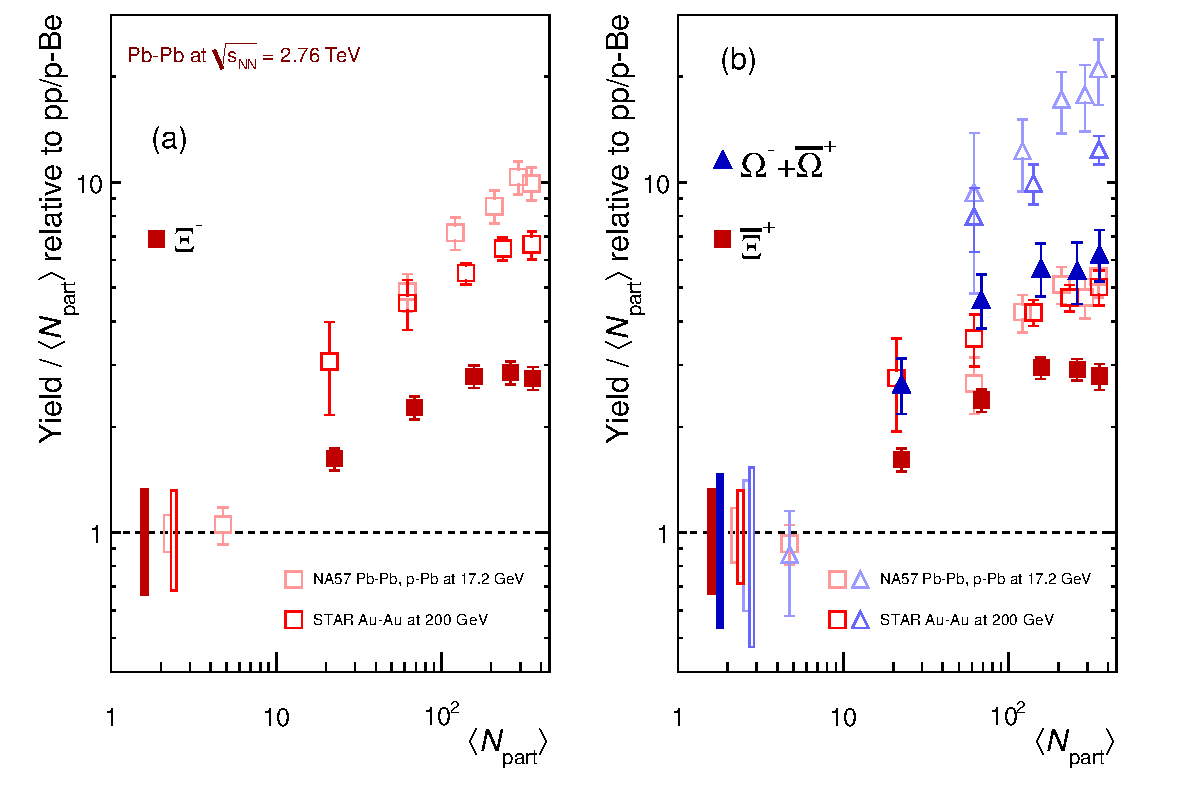
\includegraphics[width=12.cm]{./Version1/FigChapter3/MultdNdy}
\caption{Enhancements in the rapidity range  $\arrowvert y \arrowvert<$0.5 as a function of the mean number of participants  $\langle N_{part}\rangle$, showing LHC (ALICE, full symbols), RHIC and SPS (open symbols) data. Boxes on the dashed line at unity indicate statistical and systematic uncertainties on the pp or p-Be reference. Error bars on the data points represent the corresponding uncertainties for all the heavy-ion measurements and those for p--Pb at the SPS. }
\label{fig:dNdy}
\end{center}
\end{figure}


The measured enhancement factors of baryons with increasing strangeness content are reported in Figure \ref{fig:dNdy} as a function of the number of participant nucleons, $\langle N_{part}\rangle$, in comparison with similar measurements at SPS and RHIC. For p--Pb collisions there is no evidence of enhancement. For Pb--Pb collisions the enhancement increases with centrality and the effect is larger for particles with higher strangeness content, up to a factor ?20 for ?s. No hadronic model has reproduced these observations and they can be interpreted as clear signal of QGP state formation. The comparison with results from the previous experiments shows that the relative enhancements decrease with increasing collision energy. An explanation of this behavior is given in terms of a statistical model, with canonical strangeness conservation. In a small system, with small particles multiplicities, quantum numbers conservation laws (such as strangeness) must be applied locally, event-by-event, whereas in a large system, with many degrees of freedom, they can be applied in average, by means of the corresponding chemical potential. The conservation of quantum numbers is known to reduce the phase space available for particle production. This canonical suppression factor decreases with lower energy in the centre of mass of the collisions and could explain the larger enhancement for lower energy systems.





\subsection{Resonance production}

\begin{figure}[htbp]
\begin{center}
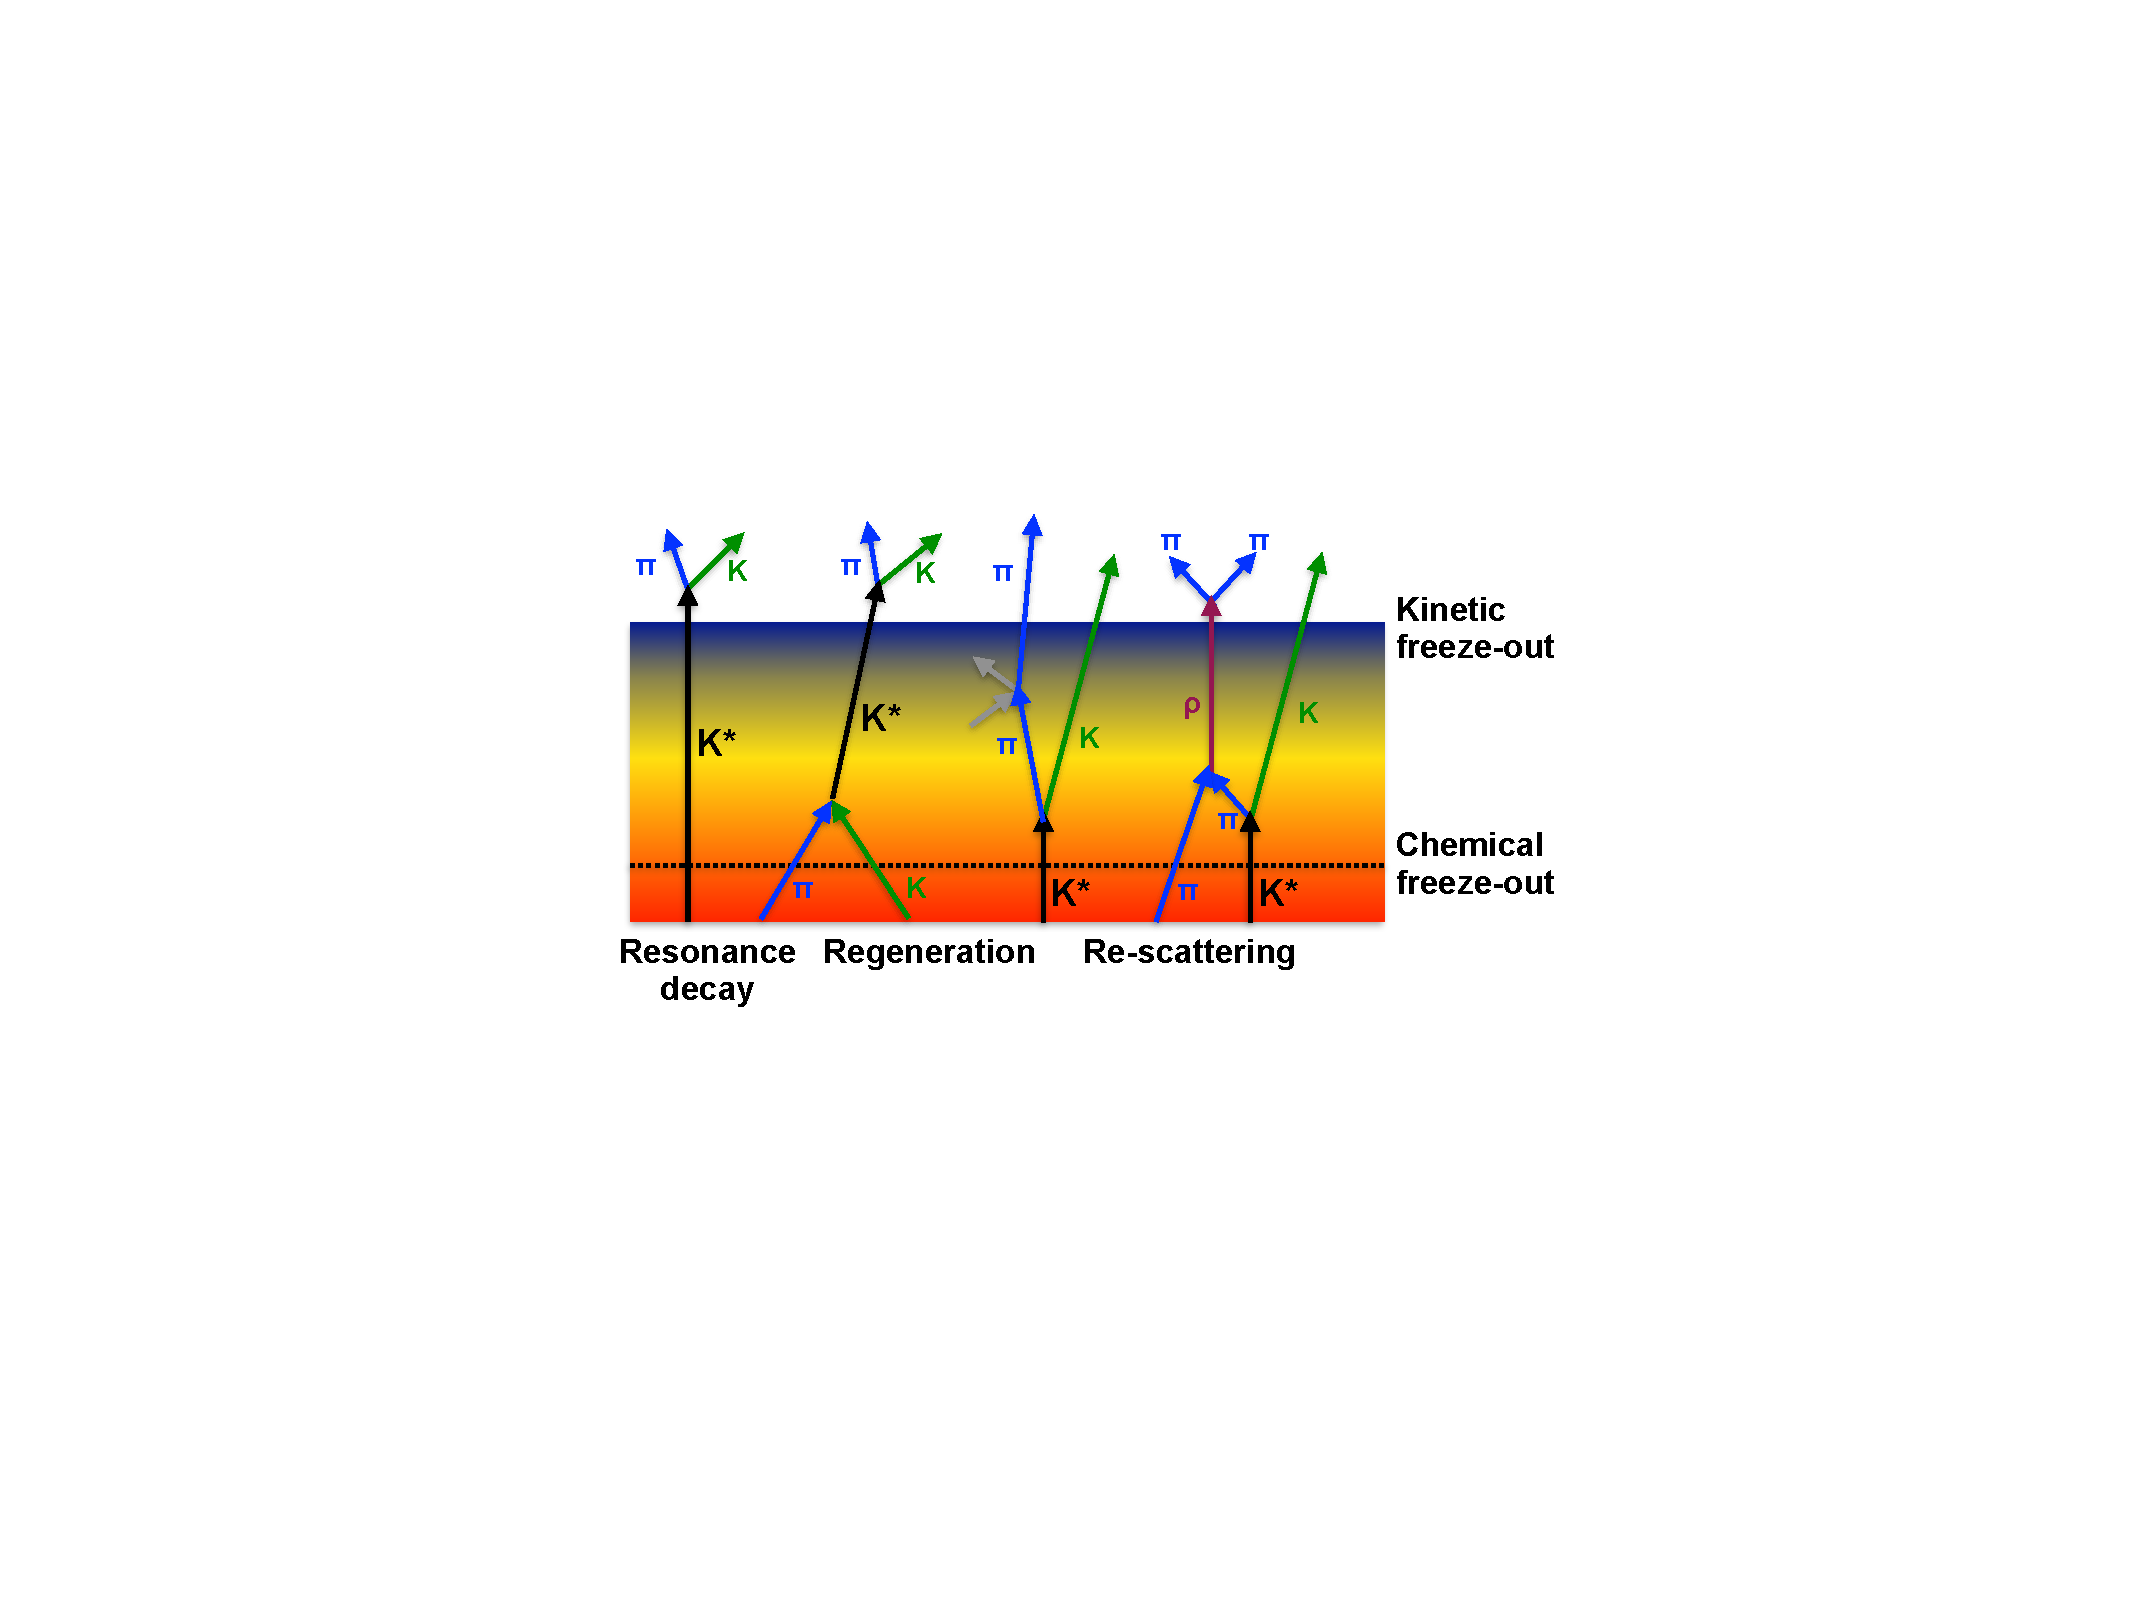
\includegraphics[width=12.cm]{./Version1/FigChapter3/Hadronic}
\caption{Hadronic phase }
\label{fig:hadronic}
\end{center}
\end{figure}


Resonances are particles with higher mass than the corresponding ground state particle with the same quark content. Hadronic resonances decay strongly, thus with a short lifetime, $\tau \sim$ few tenths of fm/c. The resonance natural width is given by $\Gamma = \bar{h}$/$\tau$, that is inversely proportional to the lifetime. Broad states with finite $\Gamma$ decay very shortly after being produced and can be measured only by reconstruction of their decay products (or "daughters") in a detector. In heavy-ion collisions, hadronic resonances are produced within the bulk of the expanding medium, where they can decay while still traversing its volume. Decay products may interact with the other particles of the medium (mostly pions at the LHC), resulting in the impossibility of reconstructing the resonance, because the invariant mass of the daughters does not match that of the parent particle. Conversely, resonances may be regenerated as a consequence of pseudo-elastic collisions in the time lapse between the chemical ($T_{ch}$) and the kinetic freeze-out ($T_{kin}$). Re-scattering and regeneration depend on the individual cross section, hence lifetime, of the resonances and affect the measurement of their yield and momentum spectrum. The yield is decreased if the re-scattering dominates, vice versa the regeneration feeds the system with more particles. The two effects may even compensate.
Different resonances with different lifetimes can probe different stages of the fireball expansion. The ratios between resonances and stable hadrons can be compared for resonances with different lifetimes and provide insights on the role of the re-scattering effect between the two freeze-out phases.


\newpage